\section{Produktegenskaper}

\subsection{Produktets funksjonelle egenskaper} 

\begin{itemize}
    \item HTTP Klient som skal hente data fra eksterne kilder der det er mulig
    \item Filleser som skal lese inn filer som inneholder data der datafangst via API ikke var mulig. Skal også kunne lese inn filer som lagres i binært format (f.eks PDF filer)
    \item Lagring service som snakker med data inn og data ut tjenestene og lagrer/henter data i en MySql database 
    \item Database for lagring av innhentet data
    \item REST API som serverer data til kvalitetsregister ved forespørsel
    \item Refresh service som poller storage service for endringer. Når det er registrert sendes det en melding til registeret om at det kan hente ny oppdatert data til sin in-memory database
    \item HTTP Klient som sender melding til kvalitetsregisteret om mulighet for oppdatering av data
    \item Distribueres som et container image for drift i Docker og Kubernetes miljø    
\end{itemize} 

Hoved logikken i applikasjonen vil ligge i en Storage Service som har ansvar for å holde på data. Den vil via jevne mellomrom prøve å automatisk oppdatere data fra eksterne kilder, samt ha evne til å motta manuelt innlastede filer. Dette gjøres via respektive HTTP- og fil-klienter Den persisterer data i en database. Applikasjonen vil ha en tjeneste som gir beskjed til register applikasjonen når ny data kan hentes fra REST apiet. Beskjeden blir gitt via et HTTP kall fra en HTTP-klient.

Tjenesten som skal kjøre i applikasjonen for å utføre periodiske oppgaver vil kjøres via såkalte coroutines. En coroutine er en type virituell tråd som kan suspenderes når den ikke jobber for så å vekkes igjen når den skal jobbe. De er et lettvekts konstrukt i Kotlin for å skrive applikasjoner som skal utføre samtidige prosseser. Med coroutines som verktøy kan vi oppnå samtidige langtids kjørende jobber som bruker minimalt med system ressurser.\cite{4-coroutines} Vi kan også benytte oss av ikke-muterende datastrukturer og metoder som kan abstrahere over de for å utføre parallelle prosesser på en trygg måte.

Http klient og lagring av koder i register kode-basen blir utviklet parallelt med applikasjonen, på denne måten kan vi vite at vi alltid kan gi og motta meldinger til
registrene som skal bruke løsningen. Register kodebasen har i dag støtte for å bruke Ktor http-klient.

Figur \ref{fig:dataflyt} viser dataflyt i applikasjonen. Grønne ruter skal implementeres som en den av prosjektet.
%Figur - Dataflyt
\begin{figure}[ht]
\centering
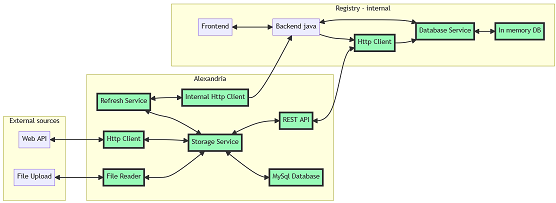
\includegraphics{images/dataflyt2.png}
\caption{Detaljert dataflyt i applikasjonen. Generert med mermaid.}
\label{fig:dataflyt}
\end{figure}

\newpage
\subsection{Ikke funksjonelle egenskaper}

Det er forventet at produktet er levert med høy kvalitet på kode, høy grad av test dekning, og godt beskrevet dokumentasjon. Det skal være lett for andre utviklere å videreutvikle produktet. Produktet skal ha et logisk konstruert API. Det må vere støtte for måling av metrics via f.eks. Prometheus. Applikasjonen må kunne settes opp med TLS for sikker kommunikasjon på helsenettet. Applikasjonen må kunne nå og kommunisere med de ulike registrene som kjører i produksjon. Det må i registeret da være mulig å sette hvilken url/ip-adresse tjenesten kjører på. Samtidig må tjenesten kunne nå de eksterne datakildene den skal snakke med for å hente data. Kommunikasjon med registre og eksterne tjenester vil skje med HTTP. Applikasjonen må da kunne tolke og behandle de ulike HTTP responsene, f.eks loggføring av Bad Request meldinger.